%----------------------------------------------------------------------------------------
%	PACKAGES AND OTHER DOCUMENT CONFIGURATIONS
%----------------------------------------------------------------------------------------

\documentclass[11pt]{article}
\usepackage{color, colortbl}
\usepackage{tabularx,ragged2e,booktabs,caption}
\usepackage[table,x11names]{xcolor}
\usepackage[utf8]{inputenc} % Required for inputting international characters
\usepackage[T1]{fontenc} % Output font encoding for international characters
\usepackage[pdftex]{graphicx}    
\usepackage{url} 
\usepackage{booktabs}
\usepackage{amsmath}
\usepackage{tabularx}
\usepackage{graphicx}
\usepackage{mathpazo} % Palatino font
\usepackage[english]{babel}

\addto\captionsenglish{% Replace "english" with the language you use
  \renewcommand{\contentsname}%
    {Sadržaj}%
}

\captionsetup[table]{name=Tablica}
\addto\captionsenglish{\renewcommand{\figurename}{Slika.}}

\begin{document}

%----------------------------------------------------------------------------------------
%	TITLE PAGE
%----------------------------------------------------------------------------------------

\begin{titlepage} % Suppresses displaying the page number on the title page and the subsequent page counts as page 1
	\newcommand{\HRule}{\rule{\linewidth}{0.5mm}} % Defines a new command for horizontal lines, change thickness here
	
	\center % Centre everything on the page
	
	%------------------------------------------------
	%	Headings
	%------------------------------------------------
	
	\textsc{\LARGE Fakultet elektrotehnike i računarstva}\\[1.5cm] % Main heading such as the name of your university/college
	
	\textsc{\Large Zavod za telekomunikacije}\\[0.5cm] % Major heading such as course name
	
	\textsc{\large Heurističke metode optimizacija}\\[0.5cm] % Minor heading such as course title
	
	%------------------------------------------------
	%	Title
	%------------------------------------------------
	
	\HRule\\[0.4cm]
	
	{\huge\bfseries Parkiranje vozila u spremištu javnog prijevoznika}\\[0.4cm] % Title of your document
	
	\HRule\\[1.5cm]
	
	%------------------------------------------------
	%	Author(s)
	%------------------------------------------------
	
	\begin{minipage}{0.4\textwidth}
		\begin{flushleft}
			\large
			{Tomislav Božurić}
			  % Your name
		\end{flushleft}
	\end{minipage}
	~
	\begin{minipage}{0.4\textwidth}
		\begin{flushright}
			\large
			 {Marin Vernier} % Supervisor's name
		\end{flushright}
	\end{minipage}
	
	% If you don't want a supervisor, uncomment the two lines below and comment the code above
	%{\large\textit{Author}}\\
	%John \textsc{Smith} % Your name
	
	%------------------------------------------------
	%	Date
	%------------------------------------------------
	
	\vfill\vfill\vfill % Position the date 3/4 down the remaining page
	
	{\large Siječanj, 2019} % Date, change the \today to a set date if you want to be precise
	
	%------------------------------------------------
	%	Logo
	%------------------------------------------------
	
	\vfill\vfill
	
\includegraphics[width=0.3\textwidth]{fer_logo.jpg}\\[1cm] % Include a department/university logo - this will require the graphicx package
	 
	%----------------------------------------------------------------------------------------
	
	\vfill % Push the date up 1/4 of the remaining page
	
\end{titlepage}

\tableofcontents
\newpage

\section{Opis problema}
U svrhu ovog projekta riješavan je problem parkiranja vozila u spremištima kompanije za javni prijevoz. Svako od vozila se smješta na prometne trake i pritom moramo imati na umu vrijeme polaska vozila iz spremišta, kako bi svako vozilo na vrijeme moglo izaći iz spremišta. Sam problem definira određena ograničenja koja je bilo potrebno zadovoljiti:
\begin{description}
  \item[$\bullet$] Vozilo se parkira na točno jednu traku.
  \item[$\bullet$] Na svaku traku se parkiraju vozila isključivo jedne serije.
  \item[$\bullet$] Svako vozilo se može parkirati isključivo na neku od traka koja pruža potrebnu infrastrukturu.
  \item[$\bullet$] Suma duljina vozila na traci ne smije premašiti kapcitet trake.
  \item[$\bullet$] Vozilu se može dodijeliti samo jedna pozicija u traci.
  \item[$\bullet$] Pozicija u redu u traci može biti dodjeljena  samo jednom vozilu.
  \item[$\bullet$] Polazak bilo kojeg vozila u traci mora biti prije polaska vozila koje slijedi u traci.
    \item[$\bullet$] Polazak svih vozila u blokirajućoj traci mora biti prije prvog vozila u blokiranoj traci.
    
Sam problem ima dva globalna cilja, prvi globalni cilj jest \textbf{minimizirati} broj različitih serija vozila u susjednim trakama, broj korištenih traka i neiskorišten prostor na korištenim trakama. Taj globalni cilj ignorira vremensku komponentu problema te ga opsijemo kao: \\
\begin{center}
  $\max p_1f_1 + p_2f_2 + p_3f_3$.\\ 
\end{center}


Drugi globalni cilj jest \textbf{maksimizirati} broj vozila s istim tipom rasporeda unutar trake, broj vozila s istim tipom rasporeda u susjednim trakama, te maksimizirati dorbu praksu glede vremenskog razmaka između dva izlaska vozila iz spremišta (idealno svaki izlazak odvojen između $[15,20]$  minuta, najmanje je prihvaljivo da su izlazci razmaknuti manje od 10 minuta).
Ovaj maksimizacijski problem možemo opisati sljedećom funkcijom:
\begin{center}
$\max r_1g_1 + r_2g_2 + r_3g_3$
\end{center}


\begin{table}[htbp]
\centering
\begin{tabular}{|>{\columncolor[gray]{0.6}}l|p{0.7\linewidth}| p{0.35\linewidth}|}
\hline
\multicolumn{1}{|c|}{\textit{\textbf{Cilj}}} & \multicolumn{1}{c|}{\textit{\textbf{Vrijednost}}} & \multicolumn{1}{c|}{\textit{\textbf{Težinski faktor}}}                                                                                                     \tabularnewline \hline
$f_1$ & broj parova susjednih korištenih traka koje se razlikuju u parkiranoj seriji vozila & $\frac{1}{p_1}$ = broj korištenih traka $-1$ \\ \hline
$f_2$ & broj korištenih traka & $\frac{1}{p_2}$ = ukupni broj traka \\ \hline
$f_3$ & suma neiskorištenog kapacitena na korištenim trakama & $\frac{1}{p_3}$ = ukupni kapacitet svih traka - ukupna duljina svih vozila \\ \hline
$g_1$ & broj parova susjednih vozila u traci s istim tipom rasporeda & $\frac{1}{r_1}$ = ukupni broj vozila u svim trakama - broj korištenih traka \\ \hline
$g_2$ & broj susjednih korištenih traka za koje vrijedi da zadnje vozilo u traci ima raspored istog tipa kao prvo vozilo u sljedećoj traci & $\frac{1}{r_2}$ = broj korištenih traka  $-1$ \\ \hline
$g_3$ & suma nagrada i penala za vremenski razmak između polazaka, za sva susjedna vozila, u svim trakama 
\begin{equation}
    n=
    \begin{cases}
      15, & \text{$10\leq  vr \leq 20 $} \\
      10, & \text{$ vr > 20 $} \\
      4\cdot(10-vr), & \text{$ vr < 10 $} \\
    \end{cases}
  \end{equation}
   & $\frac{1}{r_3}$ = 15 $\cdot$ broj evaluiranih parova (susjeda iz traka) \\ \hline
\end{tabular}
\caption{Opis komponenti funkcija}
\label{table:economicSchools}   
\end{table}






              
\end{description}
\section{Opis primijenjenog algoritma}
U svrhu rješavanja ovog projekta korištena su tri algoritma. Pohlepni algoritam, eliminacijski genetski algoritam s turnirskom selekcijom, te taboo pretraživanje u svrhu lokalnog pretraživanje nakon pronađenog rješenja koje zadovoljava gore navedena ograničenja. Na početku pomoću pohlepnog algoritma opisanog u idućem odjeljku pokušavamo razmjestiti što je više moguće vozila u trake, zatim na temelju tako dobivenog rješenja pomoću genetskog algoritma gradimo populaciju jedinku jednostavnim permutacijama, te nakon što genetskim algortmom nađemo rješenje koje zadovoljava sva ograničenja,genetski algoritam počinje koristiti funkciju evaluacije koja dodatno optimira i dobrotu rješenja, te na kraju taboo pretraživanjem lokalno pretražujemo za još bolja rješenja. Korišten je genetski eliminacijski algoritam, kao prikaz rješenja koristi se vektor permutacija cijelih nenegativnih brojeva koji označavaju parkirnu traku na koje je pojedino vozilo parkirano. Primjerice moramo li parkirati 50 vozila u spremište javnog prijevoznika, taj vektor ima 50 elemenata i svaki elemenet onačava na kojoj traci je parkirano vozilo koje je označeno indeksom u vektoru. Kao selekcija koristi se jednostavna 3-turnirska selekcija gdje se najgora jedinka eliminira iz populacije, a preostale dvije se križaju te se naposljetku dijete mutira i dodaje u populaciju. Odabrana je 3-turnirska selekcija jer se pokazala da se dobro ponaša tijekom postupka traženja rješenja i omjer preživljavanja dobrih i loših jedinki je zadovoljavajuć. Kao metode križanja implementirane su: križanje s jednom točkom prekida, križanje s više točaka prekida, te  višesturko križanje kojem preko parametra predamo željeni broj elemenata, i na temelju tog broja nasumično generiramo indekse i prilikom kreiranja nove jednike na tim indeksima uzimamo vrijednosti od drugog roditelja, dok na preostalim indeksima elemente prvog roditelja. Za mutaciju se koristi jednostavna mutacija gdje s vjerojatnosšću mutacije jedinke $p_m$ biramo nasumično element jedinke, i mijenjamo ga nekim drugom elementom, odnosno nekom drugom parkirnom trakom. Dodatno, implementirana je i metoda unifomrne mutacije, gdje iteriramo po svim elementima jedinke i s određenom vjerojatnošću uzimamo element prvog roditelja ili uzimamo element drugog roditelja. U samome radu koriste se obje vrste mutacije i svaku biramo s vjerojatnošću $0.5$. Ekvivalentno, za križanje koristimo višestruko križanje s različitim brojem elemenata koje želimo nasljediti od drugog roditelja. 
Kad genetski algoritam naše validno rješenje, nastoji mu optimirati dobrotu rješenja, odnosno maksimizirati omjer drugog i prvog cilja, te nakon toga najbolje pronađeno rjšenje predaje taboo algoritmu, koji ga koristi kao početno rješenje. Početno rješenje postavljamo kao najbolje i kao trenutno rješnje. Za trenutno rješenje generiramo susjedstvo, na način da radimo permutacije svakog vozila sa svakim. Dodatno, susjedstvno čine i rasporedi gdje premještamo vozila u prazne trake. U svakoj iteraciji evaluiramo sve tako generirane susjede i tražimo najboljeg poboljšavajućeg susjeda. Kad nađemo boljeg susjeda odabiremo njega kao trenutno rješenje i pamtimo tu izmjenu u taboo listu. Algoritam staje nakon određenog broja iteracija.
Detalji oko pojedinih heurističkih odosno evolucijskih  algoritama dani su u nastavku u tablicama. 

\begin{center}
\centering
  \begin{tabular}{ | >{\columncolor[gray]{0.6}}c | c |}
    \hline
     Prikaz rješenja & mapa u kojoj za svaku traku imamo listu vozila \\ \hline
     Funkcija cilja & evaluira se prema zadanim funkcijama cilja \\ \hline
     Funkcija prikladnosti &  evaluira se prema zadanim funkcijama cilja\\ \hline
     Početno rješenje &  rješenje koje je našao genetski algoritam\\ \hline
     Trajanje tabua &  8 iteracija\\ \hline
     Generiranje susjedstva &  sve permutacije vozila(uz popunjavanje praznih traka)\\ \hline
     Kriterij zaustavljanja & 50 iteracija \\ \hline
\end{tabular}
\captionof{table}{Taboo pretraživanje} \label{tab:title} 
\end{center}


\begin{center}
\centering

  \begin{tabular}{ | >{\columncolor[gray]{0.6}}c |c|}
    \hline
     Prikaz rješenja & vektor permutacija parkirnih traka \\ \hline
     Funkcija cilja na početku & suma svih pogrešaka koje dijele rješenje od validnog \\ 
               Nakon pronalska validnog rješenja & kao do tada + (maks.  - min. problem) \\ \hline
     Funkcija prikladnosti na početku &  suma svih pogrešaka koje dijele rješenje od validnog\\ 
     Nakon pronalaska validnog rješenja &  kao do tada + (maks.  - min. problem) \\ \hline
     Početno rješenje &  pohlepni algoritam i permutacije \\ \hline
     Selekcija &  3-turnirska selekcija\\ \hline
     Križanje &  uzimanje $n$ elemenata druge jedinke\\ \hline
     Mutacija &  uniformna mutacija i zamjena parkirne trake vozilu\\ \hline
     Vjerojatnost mutacije &  $p_m=0.03$ \\ \hline
     Veličina populacije &  10\\ \hline
     Kriterij zaustavljanja & vremensko ograničenje \\ \hline
\end{tabular}
\captionof{table}{Genetski algoritam} \label{tab:title} 
\end{center}
\newpage

Najveći problem genetskom algoritmu predstavlja pronalaženje početnog rješenja koje zadovoljava sva ograničenja. Problem su ravne plohe u funkciji optimizacije koje predstavljaju broj zadovoljenih ograničenja (primjer jedne plohe crvenom bojom na grafu), i takve ravne plohe predstavljaju težak zadatak izvlačenja iz lokalnog optimuma te je zbog toga samom genetskom algoritmu potreban nešto veći broj iteracija za pronalazak početnog validnog rješenja, no kada pronađe početno validno rješenje (plavom bojom na grafu) i kada funkciji evaluacije dodajemo dobrotu pojedinog rješenja, algoritam efikasno pronalazi sve bolje i bolje jedinke, odnosno sve bolja i bolja rješenja.
\begin{center}
\begin{figure}
  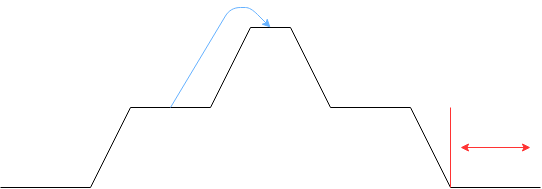
\includegraphics[width=\linewidth]{fjaOptimizacije.png}
  \caption{Optimizacijska funkcija pronalaska rješenja koje ne krši zadana ograničenja }
  \label{fig:optFun}
\end{figure}

\end{center}

\section{Pseudokod}
Pseudokod pohlepnog algoritma dan je u nastavku:


\begin{enumerate}
  \item Grupiraj vozila po seriji kojoj pripadaju.
  \item Za svaku seriju vozila izračunaj prosječan broj traka na koje se automobili iz te serije mogu parkirati.
  \item Sortiraj rastuće serije vozila po prethodno izračunatoj mjeri.
  \item Za svaku seriju iz prethodno sortirane liste dohvati vozila iz te serije i sortiraj ih rastuće po: vremenu polaska, broju parkinih traka na koje vozilo može parkirati, tipu rasporeda te zatim po identifikatoru.
  \item Za svako tako sortirano vozilo dohvati parkirne trake na koje se vozilo može parkirati i sortiraj parkirne trake rastuće po broju blokirajućih traka, pa po slobodnom prostoru na pojedinoj parkirnoj traci.
  \item Za tako sortiranu listu parkinih traka na svaku od njih pokušaj parkirati vozilo ako parkiran traka nije puna i ako se na njoj ne nalaze vozila neke druge serije.
\end{enumerate}

Pseudokod genetskog eliminacijskog algoritma i taboo algoritma je klasični pristup, pa ga ovim putem ne navodim.


\section{Rezultati}
Iz rezultata prikazanih u nastavku možemo vidjeti kako algoritam uspješno pronalazi rješenja te parkira vozila u garažu bez kršenja ograničenja. Zbog same probabilističke prirode genetskih algoritama, vrijeme pronalska rješenja varira u razumljivim intervalima. Rad genetskog algoritma isproban je na mnogo parametara se pokazalo da najbolja rješenja pronalazi za malu vjerojatnost mutacije (otprilike $1-3\%$). Također se pokazalo da za veće veličine populacije nismo dobili na kvaliteti rješenja, pa samim time zbog većeg broj operacija koje je potrebno izvesti kod veće populacije, korištena je manja populacija koja je davala rješenja jednake ili bolje kvalitete u kraćem vremenu. Bilo je potrebno dosta pripaziti na operatore križanja i mutacije zbog vrlo ograničenog problema, pa samim time je razumljivo da vjerojatnost mutacije se očekuje da bude malena (kao što je i uobičajeno), a da operatorom križanja ne izgubimo dobar genetski materijal od roditelja ili u drugoj krajnosti da nasumično pretražujemo. Također, zbog zadanih ograničenja genetskom algoritmu treba nešto više iteracija da evaluira k dobrim rješenjima, pa je bilo potrebno u svakom koraku pamtiti što je više prethodno izračunatih operacija kako nebi bespotrebno trošili procesorsko vrijeme. Eliminacijski genetski algoritam jest nakon 1 minute izmijenio 70 000 generacija, dok je za 5 min napravio 350 000 generacija. Za prvu instancu za "beskonačno" prvu instancu smo najduže izvodili i izmijenili 9 000 000 generacija,  drugu instancu 4 000 000 generacija te za treću instancu 5 900 000 generacija. Genetski algoritam nije evoluirao funkciju cilja dok nije pronašao inicijalno rješenje koje zadovoljava sva postavljena ograničenja.

\begin{center}
\centering

  \begin{tabular}{ | >{\columncolor[gray]{0.6}}c|c|c|c| }
    \hline
  	Broj minuta & nakon 1 minute & nakon 5 minuta & beskonačno \\ \hline
  	$f_1$ & 0.25 & 0.25 & 0.25 \\ \hline 
  	$f_2$ & 0.86206895 & 0.86206895 & 0.86206895 \\ \hline 
  	$f_3$ &  0.3174716 & 0.30610797 & 0.30042616 \\ \hline 
  	$g_1$ &  0.5833334 & 0.625 & 0.75 \\ \hline 
  	$g_2$ & 0.7083334 & 0.7916667 &  0.9166667 \\ \hline 
  	$g_3$ & 0.8 &  0.78933334 & 0.8933333 \\ \hline 
  	$cilj_1$  & 1.4295405 & 1.4181769 &  1.412495\\ \hline 
  	$cilj_2$ & 2.0916667 & 2.206 & 2.56 \\ \hline 
  	$omjer$ & 1,463174356 & 1,555518215 & 1,812395796 \\ \hline 
\end{tabular}
\captionof{table}{Rezultati prve instance} \label{tab:title} 
\end{center}


\begin{center}
\centering

  \begin{tabular}{ | >{\columncolor[gray]{0.6}}c|c|c|c| }
    \hline
  	Broj minuta & nakon 1 minute & nakon 5 minuta & beskonačno \\ \hline
  	$f_1$ & 0.3846154& 0.3846154 &  0.34615386 \\ \hline 
  	$f_2$ &0.9310345 & 0.9310345 & 0.9310345 \\ \hline 
  	$f_3$ &0.64624506 & 0.6284585 & 0.6185771 \\ \hline 
  	$g_1$ & 0.61538464 &  0.7692308& 0.8846154 \\ \hline 
  	$g_2$ & 0.5769231 & 0.7692308 &  0.7692308 \\ \hline 
  	$g_3$ &  0.7820513& 0.82051283 & 0.8717949 \\ \hline 
  	$cilj_1$  & 1.961895 & 1.9441084 &  1.8957654 \\ \hline 
  	$cilj_2$ & 1.974359&  2.3589745 & 2.5256412 \\ \hline 
  	$omjer$ & 1,006353041 & 1,213396588 & 1,332254086 \\ \hline 
\end{tabular}
\captionof{table}{Rezultati druge instance} \label{tab:title} 
\end{center}


\begin{center}
\centering
  \begin{tabular}{ | >{\columncolor[gray]{0.6}}c|c|c|c| }
    \hline
  	Broj minuta & nakon 1 minute & nakon 5 minuta & beskonačno \\ \hline
  	$f_1$ & -& -& 0.4814815 \\ \hline 
  	$f_2$ & -& -& 0.9655172 \\ \hline 
  	$f_3$ & -& -& 0.82114625 \\ \hline 
  	$g_1$ & -& -& 0.79999995 \\ \hline 
  	$g_2$ & -& -&  0.8518519 \\ \hline 
  	$g_3$ & -& -& 0.8666667 \\ \hline 
  	$cilj_1$  & -& -&  2.268145\\ \hline 
  	$cilj_2$ & -& -& 2.5185184 \\ \hline 
  	$omjer$ & -& -& 1,110386858 \\ \hline 
\end{tabular}
\captionof{table}{Rezultati treće instance} \label{tab:title} 
\end{center}


\section{Zaključak}
Projekt se pokazao kao dosta izazovan i bilo je zanimljivo vidjeti kako u praksi izgleda rješavanje nekog tako ograničavajućeg problema. S obzirom da genetski algoritam se može vrlo različito ponašati za male promjene u parametrima, kao prijedlog jednog od daljnih poboljšanja bi bilo provođenje statistike za različite paremetre genetskog algoritma i uzimanjem najbolje prosječne vrijednosti odrediti optimalne parametre incijalno implementiranog genetskog algoritma. U svrhu dodatnog poboljšanja vremena potrebnog za pronalazak rješenja mogli bismo u više dretvi pokrenuti više instanci odnosno napraviti \textit{thread-poll} te pratiti u određenim vremenskim razmacima napredovanje pojedine instance i onu najbolju ostaviti aktivnom.

%----------------------------------------------------------------------------------------

\end{document}
